\documentclass[fullscreen=true, unicode, bookmarks=false]{beamer}
\usepackage[T2A]{fontenc}
\usepackage[utf8]{inputenc}
\usepackage[english, russian]{babel}
\usepackage{amsmath}
\usepackage{amsmath,amsfonts,amssymb}
\usepackage[export]{adjustbox}
\usepackage{textgreek}
\newtheorem{rustheorem}{Теорема }[subsection]
\newtheorem{ruslemma}{Лемма }[subsection]
\sloppy

\setbeamertemplate{navigation symbols}{}

\DeclareMathOperator{\arsh}{arsh}

\usetheme{Madrid}

\usecolortheme{whale}

\usefonttheme{professionalfonts} % default family is serif

\setbeamertemplate{footline}{\hspace*{.5cm}\scriptsize{\insertshorttitle
\hspace*{50pt} \hfill\hspace*{.5cm}}\vspace{5pt}} 

\setbeamercolor{bibliography entry author}{fg=black}

\title[]{ {\huge Потеря устойчивости нулевого состояния равновесия одной краевой задачи с дополнительной внутренней связью } }   
\author[]{{\large Л.И.~Ивановский}} 
\date{ }
\institute[]
{ ЯрГУ им. П.Г. Демидова

Объединенный институт математики и компьютерных наук им. А.Н. Колмогорова }

\begin{document}

\begin{frame}
\titlepage
\end{frame} 

\begin{frame}
\frametitle{ Система стабилизации температуры }
 
\begin{equation}
\dot{T} = T'',
\end{equation}
\begin{equation}
T(0, t) \, = 0, \quad T'(1, t) \, = f(1 - T (x_0, t)) \sigma (1 - T (x_0, t)), 
\end{equation}	

$$ t \geqslant 0, \quad x \in [0,1], \quad x_0 \in [0, 1] $$

\begin{exampleblock}{}
Rudyi A.S. Theoretical Fundamentals of the Method for Thermal Diffusivity Measurements from Auto-Oscillation Parameters in a System with a Thermal Feedback // International Journal of Thermophysics, 1993, vol. 14, no. 1, pp. 159 -- 172.
\end{exampleblock}

\end{frame}

\begin{frame}
\frametitle{  Физическая модель системы стабилизации}

\begin{figure}[ht]
\begin{minipage}[h]{0.99\linewidth}
\center{\includegraphics[scale=0.3]{images/Rudyi_model.png} }
\end{minipage}
1) Распределенный объект управления, 2) петля обратной связи, 3) контроллер, 4) источник энергии, 5) термостат
\end{figure}

\end{frame}

\begin{frame}
\frametitle{ Система стабилизации температуры }

$$ f\equiv\left(1 - T\left(\frac{1}{2}, t \right)\right)^2 $$

\begin{exampleblock}{}
Rudyi A.S. Self-excited oscillations in a parabolic system with nonlinear external feedback // Tech. Phys., 1997, vol.42, no. 5, pp. 561 -- 563.
\end{exampleblock}

\end{frame}

\begin{frame}
\frametitle{ Система регулирования температуры }
 
\begin{equation}
\dot{T} = \beta \, T'' + f(T),
\end{equation}
\begin{equation}
T'(0, t) \, = 0, \qquad T'(1, t) \, = \alpha\,T(x_0, t).
\end{equation}

$$ t \geqslant 0, \quad x \in [0,1] $$
$$ \beta > 0, \quad x_0 \in [0, 1] $$

\bigskip

$$ \tau = \beta t $$

\end{frame}

\begin{frame}
\frametitle{  Физическая модель системы регулирования}

\begin{figure}[ht]
\begin{minipage}[h]{0.99\linewidth}
\center{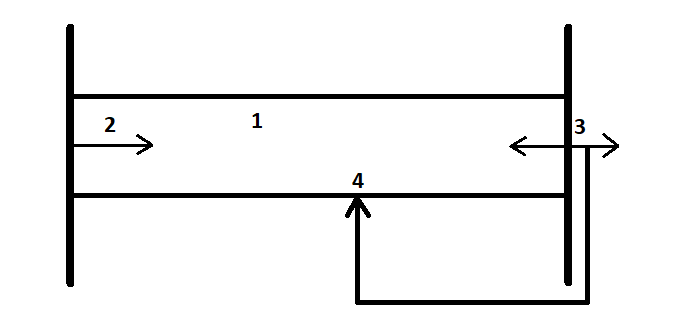
\includegraphics[scale=0.5]{images/Physical_model.png} }
\end{minipage}
1) стержень, 2) направление распространения тепла от источника, 3) точка выхода тепла, 4) точка измерения температуры на стержне, которая определяет обратную связь
\end{figure}

\end{frame}

\begin{frame}
\frametitle{ Моделирование биологического процесса }

\begin{equation}
\dot{N} = \beta \, N'' + r(1 - N^2)N,
\end{equation}
\begin{equation}
N'(0, t) \, = 0, \qquad N'(1, t) \, = \alpha\,N(x_0, t-\tilde{T}),
\end{equation}

$$ t \geqslant 0, \quad x \in [0,1] $$
$$ \tilde{T} > 0, \quad x_0 \in [0, 1] $$

\end{frame}

\begin{frame}
\frametitle{ Краевая задача с отклонением в краевом условии }
 
\begin{equation}
	\dot u = u'' + \gamma u,	
\end{equation}

\begin{equation}
	u'(0, t) \, = 0, \qquad u'(1, t) \, = \alpha\,u(x_0, t) + \beta u^3(x_0, t),
\end{equation}

\bigskip

$$ t \geqslant 0, \quad x \in [0,1]. $$

$$ \alpha, \beta, \gamma \in \mathbb{R}, \quad x_0 \in [0, 1). $$

\bigskip

\begin{exampleblock}{}
Ивановский Л.И. Динамика одной системы диффузионно связанных дифференциальных уравнений с дополнительной внутренней связью // Известия высших учебных заведений. Поволжский регион. Физико-математические науки, 2020, № 3 (55). С. 15–30.
\end{exampleblock}

\end{frame}

\begin{frame}
\frametitle{ Краевая задача с дополнительной внутренней связью }
 
\begin{equation}
	\dot u = u'' + \gamma u - u^3,	
\end{equation}

\begin{equation}
	u'(0, t) \, = 0, \qquad u'(1, t) \, = \alpha\,u(x_0, t),
\end{equation}

\bigskip

$$ t \geqslant 0, \quad x \in [0,1]. $$

$$ \alpha, \gamma \in \mathbb{R}, \quad x_0 \in [0, 1). $$

\end{frame}

\begin{frame}
\frametitle{ Цепочка уравнений с диффузионным взаимодействием }
 
\begin{equation}
	\dot u_j = N^2(u_{j+1} - 2u_j + u_{j-1}) + \gamma u_j - u_j^3, \qquad j = \overline{1, N},
\end{equation}

\begin{equation}
	u_0 = u_1, \; u_{N+1} = u_N + \dfrac{\alpha}{N}u_k, \qquad 1 \leqslant k < N,
\end{equation}

\bigskip

$$ u_j = u_j(t), \quad t \geqslant 0, \quad \alpha, \gamma \in \mathbb{R}. $$

\bigskip

\begin{figure} 
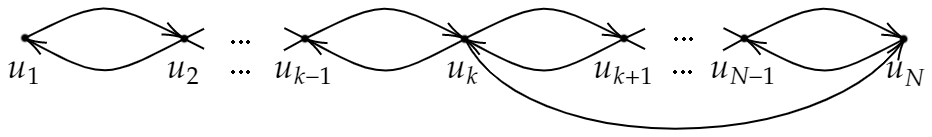
\includegraphics[scale=0.47]{u_j.png}  
\end{figure}

\end{frame}

\begin{frame}
\frametitle{ Линеаризованная в нуле система уравнений }
 
\begin{equation}
	\dot{u}_j =  N^2(u_{j+1} - 2u_j + u_{j-1}) + \gamma u_j, \qquad j = \overline{1, N},
\end{equation}

\bigskip

\begin{equation}
	u_0 = u_1, \quad u_{N+1} = u_N + \dfrac{\alpha}{N}u_k, \qquad 1 \leqslant k < N,
\end{equation}

\end{frame}

\begin{frame}
\frametitle{ Построение характеристического уравнения }
 
$$ u_j = e^{\lambda t} \ch \delta x_j, $$

$$ x_j = -\dfrac{1}{2N} + \dfrac{j}{N}. $$

\bigskip

\begin{itemize}

\item { $ j \leqslant N-1: $ 
}
\begin{equation}
\delta = 2N \arsh \dfrac{\sqrt{-\gamma+\lambda}}{2N}.
\end{equation}
\medskip
\item { $ j = N: $ 
}
\begin{equation}
\alpha = \dfrac{\sqrt{-\gamma+\lambda}\sh\delta}{\ch\delta x_k}.
\end{equation}

\end{itemize}

\end{frame}

\begin{frame}
\frametitle{ Потеря устойчивости нулевого решения }

\begin{itemize}

\item { $ \lambda = 0: $ 
}

\begin{equation}
\alpha_u = \frac{ \sqrt{-\gamma} \, \sh \delta_u }{ \ch\delta_u x_k },.
\end{equation}
$$ \delta_u = 2N \arsh \dfrac{\sqrt{-\gamma}}{2N} $$

\medskip

\item { $ \lambda = \pm i \omega: \; $ 
}

\begin{equation}
\alpha_c = \frac{ \sqrt{-\gamma + i \omega} \, \sh \delta_c }{ \ch\delta_c x_k }, 
\end{equation}
$$ \delta_c = 2N \arsh \dfrac{\sqrt{-\gamma + i \omega}}{2N}. $$

\bigskip

$$ N=50 $$

\end{itemize}

\end{frame}

\begin{frame}
\frametitle{ Предельный случай }

$$ N \rightarrow \infty: \qquad \delta \rightarrow \sqrt{-\gamma + \lambda}. $$

\bigskip

\begin{equation}
\alpha = \dfrac{\sqrt{-\gamma+\lambda}\sh\sqrt{-\gamma+\lambda}}{\ch\sqrt{-\gamma+\lambda}\:x_0}.
\end{equation}

\bigskip

\begin{itemize}

\item { $ \lambda = 0: $ 
}

$$ \alpha_u = \frac{ \sqrt{-\gamma} \, \sh \sqrt{-\gamma} }{ \ch \sqrt{-\gamma} x_0 }. $$

\item { $ \lambda = \pm i \omega: $ 
}

$$ \alpha_c = \frac{ \sqrt{-\gamma + i \omega} \, \sh \sqrt{-\gamma + i \omega} }{ \ch \sqrt{-\gamma + i \omega} x_0 }. $$

\end{itemize}	

\end{frame}

\begin{frame}
\frametitle{ Построение зависимости $ \alpha_c(\gamma) $ }
 
\begin{itemize}

\item { $ \gamma = 0, \, x_0 = 0: $ 
\begin{equation}
 \begin{cases}
   \tg \, y + \th \, y = 0, 
   \\
   \alpha_c = y(\sh y \cos y - \ch y \sin y),
 \end{cases}
\end{equation}
$$ y = \sqrt{ \frac{\omega}{2} }. $$
}

\item { $ \gamma = 0, \, x_0 \neq 0: $ 
\begin{equation}
 \begin{cases}
   \dfrac{\sh y \cos y + \ch y \sin y}{\sh y \cos y - \ch y \sin y} - \tg y x_0 \th y x_0 = 0, 
   \vspace{0.1cm}
   \\ 
   \alpha_c = \dfrac{y \sh y \cos y - y \ch y \sin y}{\ch y x_0 \cos y x_0}.
 \end{cases}
\end{equation}
}

\item { $ \gamma \neq 0, \, x_0 \neq 0. $ 
}

\end{itemize}	

\end{frame}

\begin{frame}
\frametitle{ Численные результаты: $ \alpha_c(x_0) $ при $ \gamma = 0 $ }

\begin{figure} 
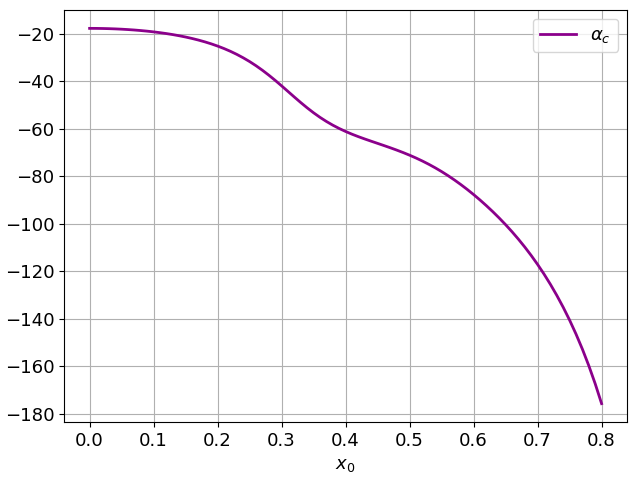
\includegraphics[scale=0.65]{origins.png}  
\end{figure}

\end{frame}

\begin{frame}
\frametitle{ Визуализация критических зависимостей }

\begin{center}
\begin{tabular}{cc}
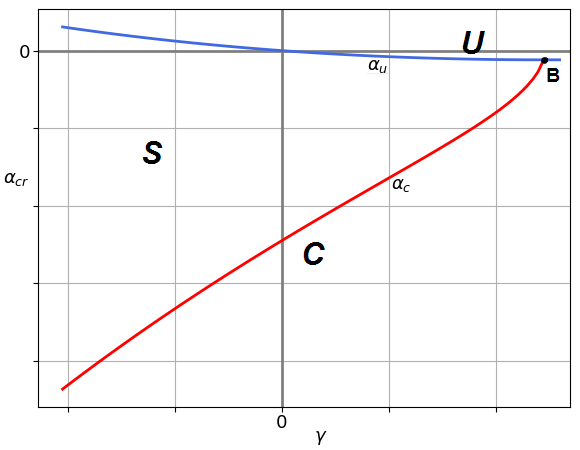
\includegraphics[scale=0.35]{images/k=1.png} &
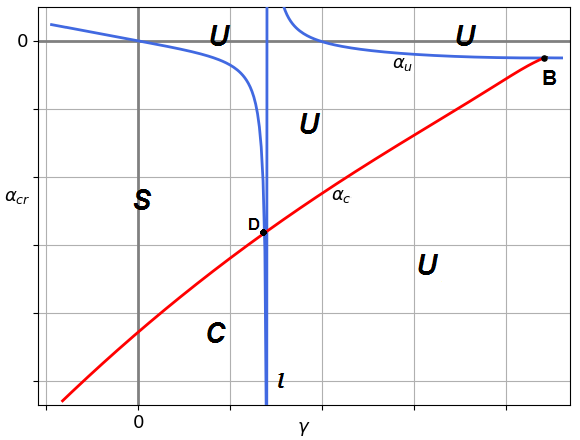
\includegraphics[scale=0.35]{images/k=26.png} \\
а) $k=1 \; (x_0=0.01)$ & б) $k=26 \; (x_0=0.51)$ \\
\end{tabular}
\end{center}

$$ B=(\gamma_*, \alpha_*): \quad \gamma_*>0, \; \alpha_*<0 $$
$$ D=(\hat{\gamma}, \hat{\alpha}): \quad 0 < \hat{\gamma} < l, \; \hat{\alpha}<0 $$

\end{frame}

\begin{frame}
\frametitle{ Визуализация критических зависимостей }

\begin{center}
\begin{tabular}{cc}
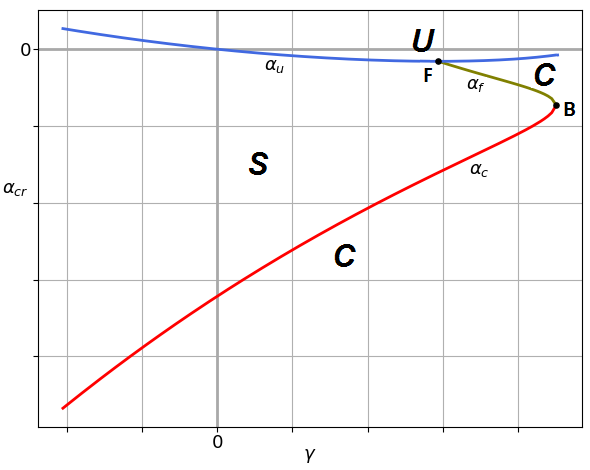
\includegraphics[scale=0.35]{images/k=22.png} &
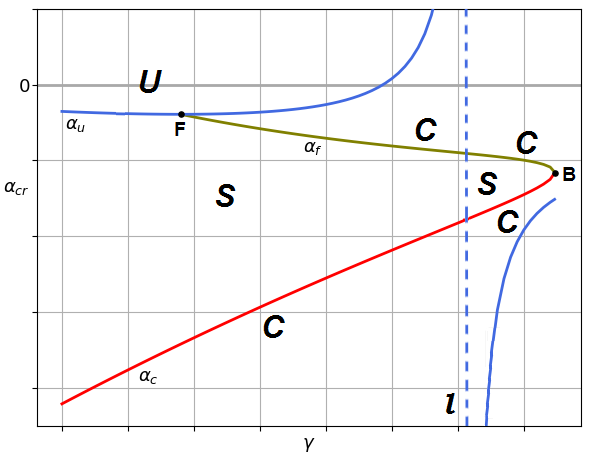
\includegraphics[scale=0.35]{images/k=24.png} \\
а) $k=22 \; (x_0=0.43)$ & б) $k=24 \; (x_0=0.47)$ \\
\end{tabular}
\end{center}

$$ F=(\overline{\gamma}, \overline{\alpha}): \quad 0<\overline{\gamma}<\gamma_*, \; 0>\overline{\alpha}>\alpha_* $$

\end{frame}

\begin{frame}
\frametitle{ Визуализация критических зависимостей }

\begin{figure} 
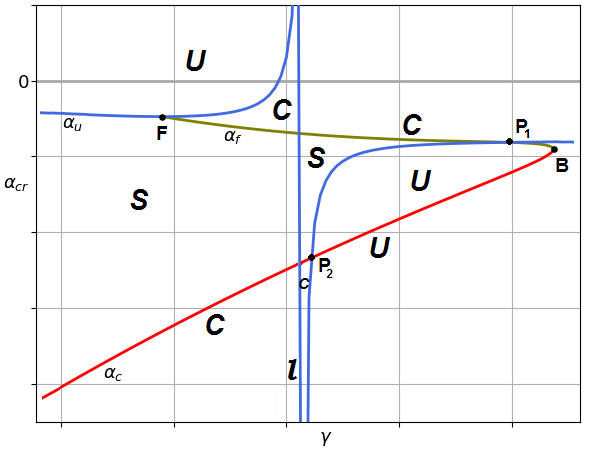
\includegraphics[scale=0.55]{images/k=25.png}  
\end{figure}
$$ k=25 \; (x_0=0.49) $$
$$ P_1=(\gamma_1, \alpha_1), P_2=(\gamma_2, \alpha_2): \quad \gamma_* > \gamma_1 > \gamma_2 > l $$

\end{frame}

\begin{frame}

\begin{equation}
    \Gamma_u =\left\{
                \begin{array}{ll}
                  \gamma_*, \quad 1 \leqslant k \leqslant 17,\\
                  \overline{\gamma}, \quad 18 \leqslant k \leqslant 25,\\
                  \hat{\gamma}, \quad 26 \leqslant k \leqslant 50.
                \end{array}
              \right.
\end{equation}

\begin{equation}
    \Gamma_f =\left\{
                \begin{array}{ll}
                  \gamma_*, \quad 18 \leqslant k \leqslant 24,\\
                  \gamma_1, \quad k = 25.
                \end{array}
              \right.
\end{equation}

\begin{equation}
    \Gamma_c =\left\{
                \begin{array}{ll}
                  \gamma_*, \quad 1 \leqslant k \leqslant 24,\\
                  \gamma_2, \quad k = 25,\\
                  \hat{\gamma}, \; \quad 26 \leqslant k \leqslant 50.
                \end{array}
              \right.
\end{equation}

\bigskip

\begin{equation}
\frac{\sqrt{-\gamma} \, \sh \delta_u}{\ch \delta_u x_{25}} - \frac{\sqrt{-\gamma + i \omega} \, \sh \delta_c}{\ch \delta_c x_{25}} = 0
\end{equation}

\end{frame}

\begin{frame}

\begin{ruslemma}
Для всех значений $\gamma \leqslant \Gamma_u$, где $\Gamma_u$ вычисляется по формуле (22) и $\gamma_1 \geqslant \gamma \geqslant \gamma_2$, где $\gamma_1, \, \gamma_2$ являются корнями трансцендентного уравнения (25), удовлетворяющими условию $\gamma_* > \gamma_1 > \gamma_2 > l$, критическая зависимость $\alpha_u(\gamma)$, рассчитываемая по формуле (17), позволяет выделить область параметров $(\gamma, \, \alpha)$ с устойчивым нулевым решением системы (11), (12) и области с двумя состояниями равновесия в малой окрестности неустойчивого нулевого решения.
\end{ruslemma}

\begin{ruslemma}
Для всех значений $\overline{\gamma} \leqslant \gamma \leqslant \Gamma_f$, где $\Gamma_f$ вычисляется по формуле (23), и $\gamma \leqslant \Gamma_c$, где $\Gamma_c$ вычисляется по формуле (24), критические зависимости $\alpha_f(\gamma)$ и $\alpha_c(\gamma)$, рассчитываемые из уравнения (18), позволяют выделить область параметров $(\gamma, \, \alpha)$ с устойчивым нулевым решением системы (11), (12) и области, для которых наблюдается наличие цикла в малой окрестности неустойчивого нулевого решения.
\end{ruslemma}

\end{frame}

\begin{frame}
\frametitle{ Локальный анализ системы }

\begin{equation}
	u_j = \sqrt{\varepsilon}u_{j,0} + \varepsilon u_{j,1} + \varepsilon^{\frac{3}{2}} u_{j,2} + O(\varepsilon^2), \qquad j = \overline{1, N}.
\end{equation}

\bigskip

$$ u_j = u_j(s), \quad s = \varepsilon t, $$

$$ \varepsilon = | \alpha - \alpha_{cr} |, \quad \varepsilon \ll 1.  $$

\end{frame}

\begin{frame}
\frametitle{ Случай дивергентной потери устойчивости }

\begin{itemize}
\item { $ \lambda = 0: \quad \varepsilon=\alpha-\alpha_u, $
}
\end{itemize}

\bigskip

\begin{equation}
	\dot u_{j,0} = N^2(u_{j+1,0} - 2u_{j,0} + u_{j-1,0}) + \gamma u_{j,0},
\end{equation}
\begin{equation}
	u_{0,0} = u_{1,0}, \quad u_{N+1,0} = u_{N,0} + \dfrac{\alpha_u}{N}u_{k,0}, \qquad 1 \le k < N
\end{equation}

\bigskip

$$ u_{j,0} = \rho(s) \ch \delta_u x_j, $$

\bigskip

$$ \alpha_u = \frac{ \sqrt{-\gamma} \, \sh \delta_u }{ \ch\delta_u x_k }, \quad \delta_u = 2N \arsh \dfrac{\sqrt{-\gamma}}{2N}, \quad x_j = -\dfrac{1}{2N} + \dfrac{j}{N}. $$

\end{frame}

\begin{frame}
\frametitle{ Случай дивергентной потери устойчивости }

\begin{equation}
	\dot u_{j,2} + \frac{\partial u_{j,0}}{\partial s} = N^2(u_{j+1,2} - 2u_{j,2} + u_{j-1,2}) + \gamma u_{j,2} - u_{j,2}^3,
\end{equation}
\begin{equation}
	u_{0,2} = u_{1,2}, \quad u_{N+1,2} = u_{N,2} + \dfrac{\alpha_u}{N}u_{k,0},
\end{equation}

\bigskip

$$ u_{j,2} = \ch \delta_u x_j. $$

\end{frame}

\begin{frame}
\frametitle{ Случай дивергентной потери устойчивости }

\begin{equation}
	\rho' = \phi_0 \rho + d_0 \rho^3,
\end{equation}

\bigskip

\begin{equation}\label{phi0_div}
\phi_0 = \frac{ 2 \delta_u \ch \delta_u x_k }{ \delta_u \ch \delta_u +\sh \delta_u - \alpha_u x_k \sh \delta_u x_k },
\end{equation}

\begin{equation}\label{d0_div}
d_0 = \frac{ 3\delta_u^2 \sh 3\delta_u - \alpha_u \delta_u \ch 3\delta_u x_k }{ 16( \delta_u \ch \delta_u +\sh \delta_u - \alpha_u x_k \sh \delta_u x_k ) } - \frac{3}{4}.
\end{equation}

\end{frame}

\begin{frame}
\frametitle{ Графики $ \phi_0(\gamma) $ и $ d_0(\gamma) $ }

\begin{figure} 
\begin{minipage}[h]{0.49\linewidth}
\begin{center}
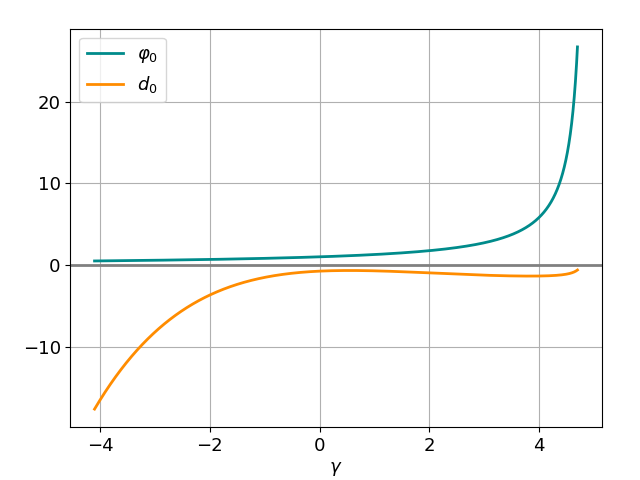
\includegraphics[scale=0.35]{images/divergent_phi0d0_033.png} \\ (а) $ k=17 \; (x_0=0.33) $
\end{center}
\end{minipage} 
\hfill
\begin{minipage}[h]{0.49\linewidth}
\begin{center}
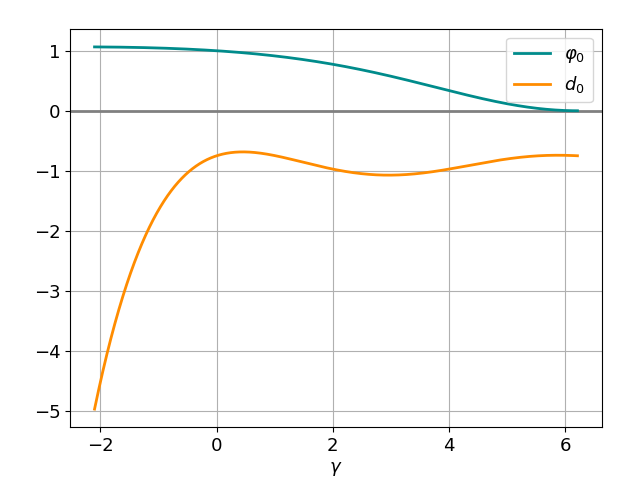
\includegraphics[scale=0.35]{images/divergent_phi0d0_063.png}  \\ (б) $ k=32 \; (x_0=0.63) $
\end{center}
\end{minipage} 
\end{figure}

\end{frame}

\begin{frame}
\frametitle{ Графики $ d_0(\gamma) $ }

\begin{figure} 
\begin{minipage}[h]{0.49\linewidth}
\begin{center}
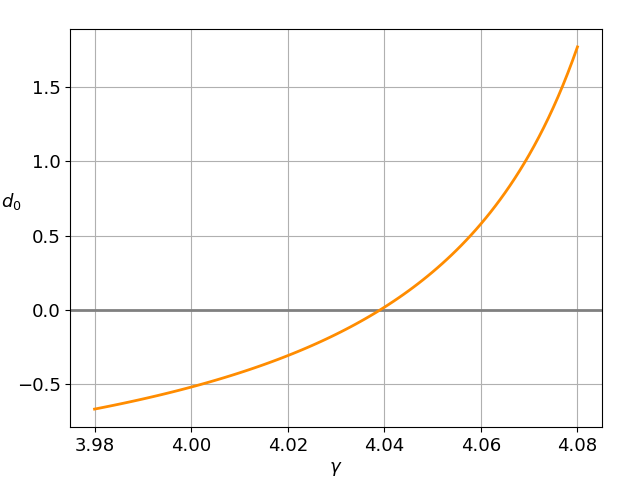
\includegraphics[scale=0.35]{images/divergent_d0_000.png} \\ (а) $ k=1 \; (x_0=0.01), \; \gamma_*\approx 4.116 $
\end{center}
\end{minipage} 
\hfill
\begin{minipage}[h]{0.49\linewidth}
\begin{center}
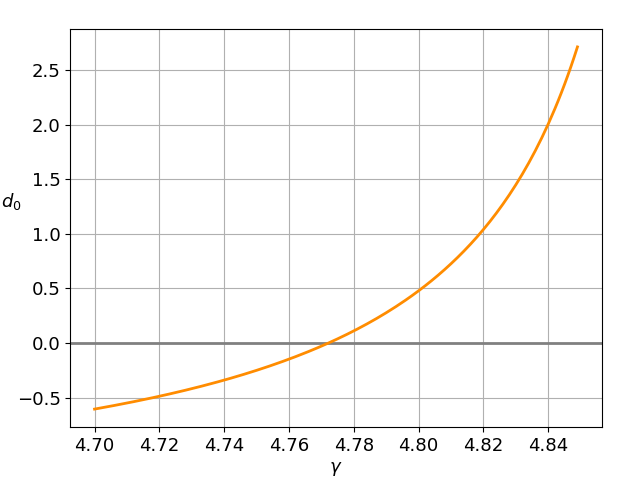
\includegraphics[scale=0.35]{images/divergent_d0_033.png}  \\ (б) $ k=17 \; (x_0=0.33), \; \gamma_*\approx 4.896 $
\end{center}
\end{minipage} 
\end{figure}

\end{frame}

\begin{frame}
\frametitle{ Графики $ d_0(\gamma) $ }

\begin{figure} 
\begin{minipage}[h]{0.49\linewidth}
\begin{center}
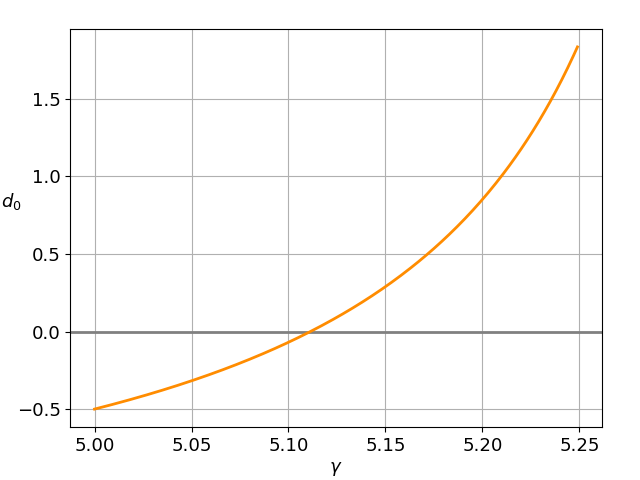
\includegraphics[scale=0.35]{images/divergent_d0_039.png} \\ (а) $ k=20 \; (x_0=0.39), \quad \overline{\gamma}\approx 5.375 $
\end{center}
\end{minipage} 
\hfill
\begin{minipage}[h]{0.49\linewidth}
\begin{center}
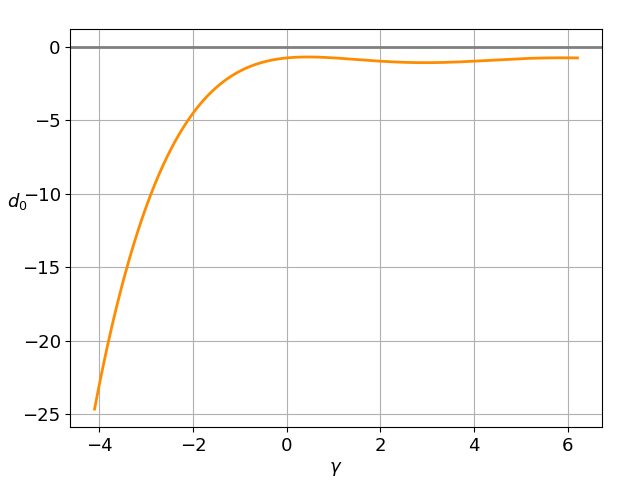
\includegraphics[scale=0.35]{images/divergent_d0_063.png}  \\ (б) $ k=32 \; (x_0=0.63), \quad l \approx 6.217 $
\end{center}
\end{minipage} 
\end{figure}

\end{frame}

\begin{frame}
\frametitle{ Случай колебательной потери устойчивости }

\begin{itemize}
\item { $ \lambda = \pm i \omega: \quad \varepsilon=\alpha_c-\alpha, $
}
\end{itemize}

\bigskip

\begin{equation}
	\dot u_{j,0} = N^2(u_{j+1,0} - 2u_{j,0} + u_{j-1,0}) + \gamma u_{j,0},
\end{equation}
\begin{equation}
	u_{0,0} = u_{1,0}, \quad u_{N+1,0} = u_{N,0} + \dfrac{\alpha_c}{N}u_{k,0}, \qquad 1 \le k < N
\end{equation}

\bigskip

$$ u_{j,0} = z(s) e^{i \omega t} \ch \delta_c x_j + \overline{z(s)} e^{-i \omega t} \overline{\ch \delta_c x_j}, $$

\bigskip

$$ \alpha_c = \frac{ \sqrt{-\gamma + i \omega} \, \sh \delta_c }{ \ch\delta_c x_k }, \quad \delta_c = 2N \arsh \dfrac{\sqrt{-\gamma + i \omega}}{2N}, \quad x_j = -\dfrac{1}{2N} + \dfrac{j}{N}. $$

\end{frame}

\begin{frame}
\frametitle{ Случай колебательной потери устойчивости }

\begin{equation}
	\dot u_{j,2} + \frac{\partial u_{j,0}}{\partial s} = N^2(u_{j+1,2} - 2u_{j,2} + u_{j-1,2}) + \gamma u_{j,2} - u_{j,2}^3,
\end{equation}
\begin{equation}
	u_{0,2} = u_{1,2}, \quad u_{N+1,2} = u_{N,2} + \dfrac{\alpha_c}{N}u_{k,0}, \qquad 1 \le k < N,
\end{equation}

\bigskip

$$ u_{j,2} = e^{i \omega t} \ch \delta_c x_j. $$

\end{frame}

\begin{frame}
\frametitle{ Случай колебательной потери устойчивости }

\begin{equation}
	z' = (\phi_0 + i \psi_0) z + (d_0 + i c_0) z |z|^2,
\end{equation}

\bigskip

$$ \phi_0 = -\mbox{Re} \left(\dfrac{2 \delta_c \ch \delta_c x_k}{\delta_c\ch \delta_c + \sh \delta_c - \alpha_c x_k \sh \delta_c x_k} \right), $$

$$ d_0 = \mbox{Re} \left( \dfrac{3 \delta_c (G(\chi) + G(\eta) + 2G(\overline{\delta_c}) )}{2(\delta_c\ch \delta_c + \sh \delta_c - \alpha_c x_k \sh \delta_c x_k)} \right), $$

\bigskip

$$ \chi = \delta_c + 2 \mbox{Re}\,\delta_c, \qquad \eta = \delta_c + 2 \mbox{Im}\,\delta_c, $$

$$ G(a) = \dfrac{\alpha_c \ch a x_k - a \sh a}{a^2 - \delta_c^2}. $$

\end{frame}

\begin{frame}
\frametitle{ Графики $ \phi_0(\gamma) $ и $ d_0(\gamma) $ }

\begin{figure} 
\begin{minipage}[h]{0.49\linewidth}
\begin{center}
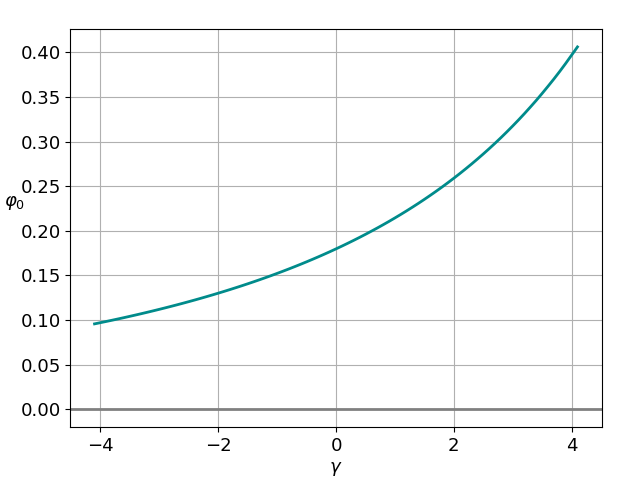
\includegraphics[scale=0.37]{images/oscillating_phi0_000.png}
\end{center}
\end{minipage} 
\hfill
\begin{minipage}[h]{0.49\linewidth}
\begin{center}
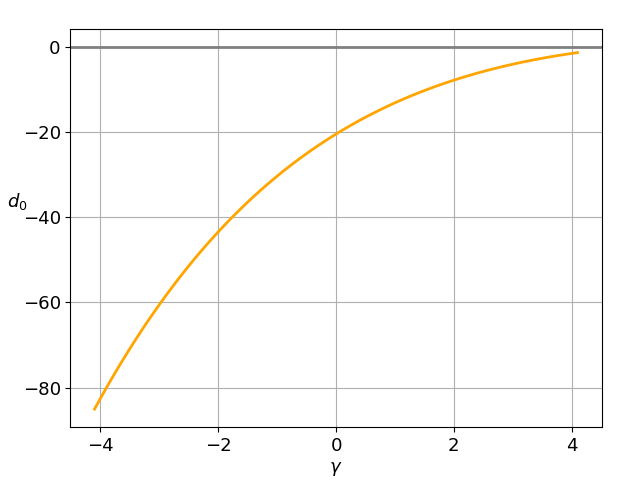
\includegraphics[scale=0.37]{images/oscillating_d0_000.png} 
\end{center}
\end{minipage} 
\end{figure}

$$ k = 1 \; (x_0=0.01), \quad \alpha_{cr}=\alpha_c $$

\end{frame}

\begin{frame}
\frametitle{ Графики $ \phi_0(\gamma) $ и $ d_0(\gamma) $ }

\begin{figure} 
\begin{minipage}[h]{0.49\linewidth}
\begin{center}
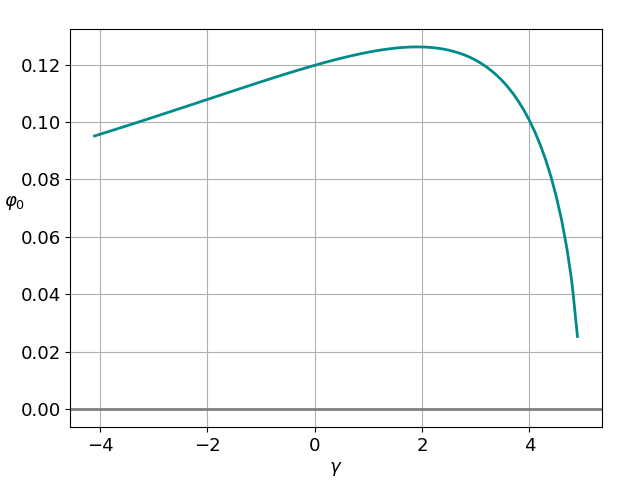
\includegraphics[scale=0.37]{images/oscillating_phi0_033.png}
\end{center}
\end{minipage} 
\hfill
\begin{minipage}[h]{0.49\linewidth}
\begin{center}
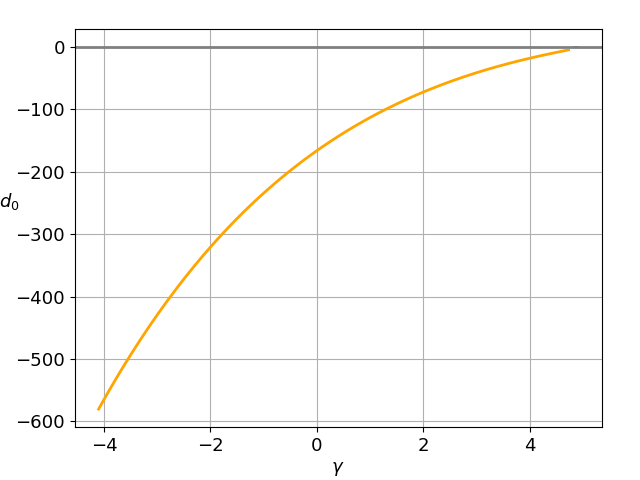
\includegraphics[scale=0.37]{images/oscillating_d0_033.png} 
\end{center}
\end{minipage} 
\end{figure}

$$ k = 17 \; (x_0=0.33), \quad \alpha_{cr}=\alpha_c $$

\end{frame}

\begin{frame}
\frametitle{ Графики $ \phi_0(\gamma) $ и $ d_0(\gamma) $ }

\begin{figure} 
\begin{minipage}[h]{0.49\linewidth}
\begin{center}
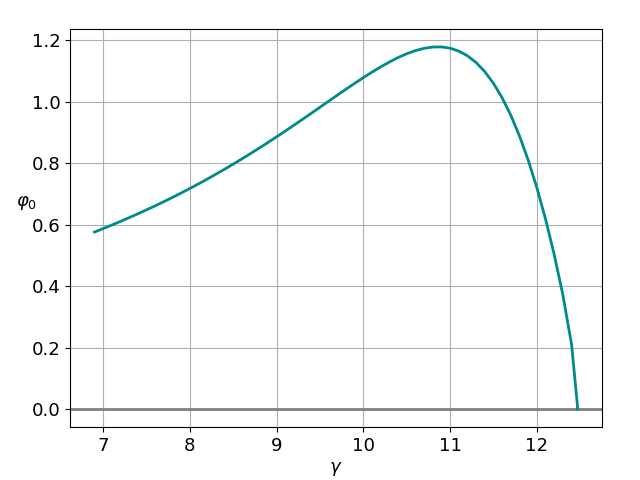
\includegraphics[scale=0.37]{images/oscillating_phi0_after_tangent_047.png}
\end{center}
\end{minipage} 
\hfill
\begin{minipage}[h]{0.49\linewidth}
\begin{center}
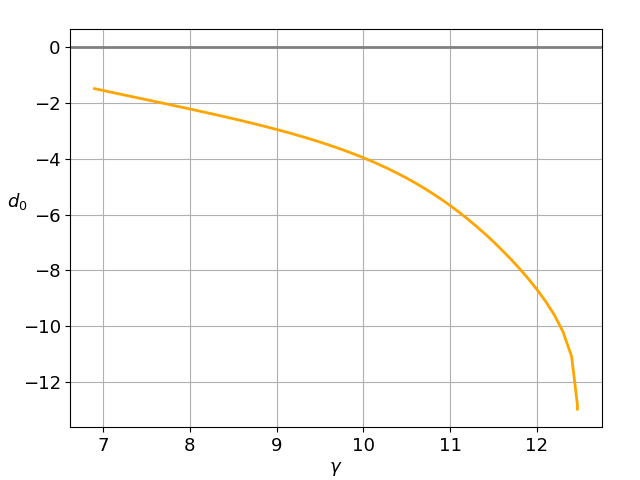
\includegraphics[scale=0.37]{images/oscillating_d0_after_tangent_047.png} 
\end{center}
\end{minipage} 
\end{figure}

$$ k = 24 \; (x_0=0.47), \quad \alpha_{cr}=\alpha_f $$

\end{frame}

\begin{frame}

\begin{rustheorem}
Для системы дифференциальных уравнений (11), (12) $\exists\;\Tilde{\gamma}<\gamma_*: \; \gamma<\Tilde{\gamma}$ нулевое состояние равновесия теряет свою устойчивость дивергентным способом.
\end{rustheorem}

\begin{rustheorem}
Для системы дифференциальных уравнений (11), (12) $\forall\;\gamma<\gamma_*$ нулевое состояние равновесия теряет свою устойчивость колебательным способом.
\end{rustheorem}

\end{frame}

\begin{frame}
\titlepage
\end{frame}

\end{document}